\chapter{DESCRIPCIÓN DE LA INVESTIGACIÓN}
\section{Planteamiento/Identificación del problema}

\subsection{Planteamiento}

La asamblea de propietarios es el órgano superior de decisión en un inmueble sometido al régimen de propiedad horizontal. Por tanto, la asamblea es un ente jurídico con personalidad jurídica propia, con la característica de estar formado por múltiples partes.

Las decisiones tomadas por la asamblea que cumplan los requisitos de ley, obliga a todos sus integrantes, ya sea que hayan estado en contra o no hayan asistido a la asamblea.

Hay que tener en cuenta que una vez adoptada una decisión, ésta ya no es individual de los copropietarios, sino de la asamblea como ente jurídico. La asamblea tiene un amplio margen de actuación, pues la ley no le pone límite a las decisiones que puede tomar, ni le hace un listado de funciones y facultades, como sí ocurre con la junta directiva. No obstante, la asamblea tiene un marco de referencia del cual no puede salirse. Ese marco de referencia es el reglamento de co-propiedad y la ley. 

Los procesos desarrollados para la planeación de las asambleas se realizan manualmente, los cuales constan de la elaboración del plan de trabajo y la divulgación del mismo, seguido se realiza la retroalimentación por parte de los copropietarios ya sea directamente en la administración o por medio de correo electrónico, lo cual dificulta la tarea cuando se habla de urbanizaciones que superan los 1000 apartamentos.

La dificultad para la toma de decisiones durante el desarrollo de la asamblea, el desconocimiento de los temas a tratar en el desarrollo de las asambleas generales, conlleva a que se convierta en una larga jornada, exasperante y fatigante, en la cual los temas que son verdaderamente importantes no sean tratados por resolver otras instancias que surgen durante la asamblea.

En el futuro estos casos se repetirán en cada asamblea lo cual seguirá generando retrasos en la preparación de las mismas, en las de la toma de decisiones, en la consolidación de resultados y en los demás subprocesos que se ven involucrados, existirán grandes cantidades de información, representadas en documentos, videos, gráficos que se encontrarán dispersos entre el archivo manejado por las administraciones de cada propiedad horizontal como evidencia de las asambleas realizadas, la generación de informes será una tarea cada vez más ardua y larga. En un mundo en auge tecnológico la no utilización de estos nuevos medios genera un retroceso que limita el crecimiento de los procesos y en este caso específico, limita que las propiedades horizontales tengan una mejor manera de realizar los procesos involucrados en las asambleas generales.

Sin un punto de control mayor al administrador y los organizadores estas jornadas pueden tardar más de 8 horas, lo cual genera retrasos en la ejecución de cada proceso, dados los problemas presentados y para incentivar el uso de las tecnologías de información, nace la necesidad de sistematizar los procesos para la ejecución de las asambleas, la cual va a permitir rapidez, fiabilidad y eficiencia en el manejo de información de las propiedades horizontales dando beneficios inherentes a los procesos.\ 
El sistema de información como tal es caracterizado por un conjunto de procedimientos organizados que se ejecutan siguiendo ciertas normas y reglas, tomando en cuenta las entradas (por medio de la captura de datos desde el prototipo de aplicación), los procesos y salida de información, las cuales se proporcionan eficientemente para la toma de decisiones y así permitir un mejor control en la organización. En este caso se hace necesario un sistema que cumpla con el requerimiento de coordinación de procesos, de tal manera que la planeación, desarrollo y entrega de información sea de forma oportuna para las asambleas generales.

\subsection{Formulación del Problema}

¿Cómo se puede sistematizar por medio de un prototipo de aplicación web el proceso de una asamblea general de copropietarios de propiedad horizontal para evitar que se convierta en una jornada larga y fatigante en su planeación, ejecución y toma de decisiones?

\subsection{Sistematización del Problema}

\begin{itemize}
\item ¿De qué forma asegurar que los temas que deben ser tratados en una asamblea general de copropietarios de propiedad horizontal sean los de su exclusiva competencia y dejar los temas generales para cada órgano competente?

\item ¿Cómo agilizar y regular el proceso de votación durante la toma de decisiones en la ejecución de la asamblea general de copropietarios de propiedad horizontal?

\item ¿Cómo generar de forma rápida y eficiente el informe de resultados de la asamblea general de copropietarios para la socialización y evaluación de la información?
\end{itemize}


\section{Objetivos}
\subsection{Objetivo General}

Construir un prototipo de aplicación web para la sistematización del proceso de asamblea general de copropietarios en propiedad horizontal mediante la implementación de servicios SOAP (Simple Object Access Protocol).

\subsection{Objetivos Especificos}

\begin{itemize}
  \item Desarrollar un módulo de planeación que le permita al usuario agilizar el proceso de preparación de las asambleas generales de copropietarios en propiedad horizontal mediante una interfaz gráfica que facilite la identificación de objetivos, los puntos del orden del día, resumir y revisar las asignaciones del día.

  \item Desarrollar un módulo de ejecución que contemple el registro y votación (Voto eléctrico desde dispositivo móvil) de los temas planificados mediante el uso de tecnología móvil para agilizar los procesos mencionados durante el desarrollo de la asamblea general de copropietarios en propiedad horizontal.

  \item Desarrollar un módulo de reportes que permita la consolidación y presentación de información recopilada mediante conteo digital y generación de informes en las asambleas generales de copropietarios en propiedad horizontal.

\end{itemize}

\section{Justificación del trabajo/investigación}

\subsection{Justificación Práctica}

En la actualidad se evidencia un aumento considerable e importante de la construcción en la modalidad de propiedad horizontal, por consiguiente, cada vez más personas deben convivir y acogerse a las normas establecidas por la ley que regula la sana convivencia en los conjuntos residenciales. 

Tomando como referencia que la Asamblea general es el órgano de dirección y control de la propiedad horizontal en la cual se deben abordar una cantidad considerable de temas que son concernientes a la convivencia y de gran importancia para toda la comunidad de residentes,  y que actualmente estas asambleas se ejecutan con grandes dificultades, se hace necesario brindar una ayuda tanto a los administradores como copropietarios de los inmuebles pertenecientes al régimen de propiedad horizontal logrando sistematizar dichas asambleas por medio de la construcción de un prototipo de aplicación con disponibilidad web y móvil mediante la implementación de servicios SOAP (Simple Object Access Protocol).  Que permitirá agilizar los procesos de preparación, registro de asistentes, votación, recopilación, consolidación y presentación de los informes de la asamblea general. Esto surge porque en las condiciones actuales del proceso de asambleas generales, los tiempos de planeación y ejecución son demasiado largos, lo cual dificulta su consolidación.

Como se ha mencionado anteriormente ante la problemática que ha surgido en las asambleas generales de copropietarios de propiedad horizontal, se proyecta desarrollar un prototipo de aplicación que permita planear, notificar con anticipación los temas a tratar, registro de asistentes, ejecutar (toma de decisiones en los cuestionamientos desarrollados en la asamblea) y en la presentación de resultados, minimizando el tiempo de conteo de votos y participación de los asistentes.

\section{Hipótesis}

Si se proporciona a las propiedades horizontales un prototipo de aplicación web que permita el desarrollo de las asambleas generales de copropietarios de manera ordenada, ágil, sencilla y eficaz, se aumentará el control y disminuirá considerablemente el tiempo en el proceso de toma de decisiones, se reducirán costos de logística, permitirá un mejor manejo de la información y generará un uso eficiente de las tecnologías de información

\newpage

\section{Marco Referencial}

\subsection{Marco Teórico}

\subsubsection{Propiedad horizontal}	

La Ley 675 de 2001 regula todo lo relacionado con la Propiedad Horizontal, que pueden ser edificios y conjuntos de uso residencial, comercial o mixto. La Propiedad Horizontal o Copropiedad Horizontal es la que tiene por finalidad tratar todos los temas referentes a esta forma de propiedad para que, posteriormente, en la eventualidad de algún inconveniente, se pueda dirimir haciendo uso de sus normas específicas.
Esta clase de propiedad cuenta con una personería jurídica, a través de escritura pública inscrita en la Oficina de Instrumentos Públicos.
La Ley 675 de 2001 regula la Propiedad Horizontal como una forma especial de dominio.  En ella se presentan derechos de propiedad exclusiva sobre unos bienes de carácter privado, pero con restricción de actividades y derechos de copropiedad sobre el terreno y sobre unos bienes denominados comunes, pero de uso privativo, tales como: pasillos, corredores, zonas de juegos, piscinas, ascensores, escaleras, salones sociales, etc.\cite{WEB1}

\begin{itemize}
\item Asamblea General de copropietarios en propiedad Horizontal

El órgano de administración más importante en una copropiedad o propiedad horizontal, trátese de un edificio o conjunto, ya sea de uso residencial, comercial o mixto, es la 
asamblea general de propietarios, que de acuerdo al precitado artículo 38, es el órgano de dirección de la persona jurídica que nace por mandato de la Ley 675 de 2001; siendo la asamblea general de propietarios, el órgano encargado de fijar las políticas y  las pautas sobre las cuales debe  funcionar el edificio o conjunto.

Debe tenerse en cuenta que, por mandato de dicha Ley, artículo 38, parágrafo, las funciones de la asamblea general de propietarios, son indelegables, pudiendo únicamente delegar en los edificios o conjuntos de uso residencia, numeral 3º del precitado artículo, la elección de los miembros para conformar el comité de convivencia.

\item Funciones de la Asamblea General de Copropietarios

La asamblea general de propietarios en edificios o conjuntos se reúne en forma ordinaria en los tres primeros meses del año con las siguientes funciones de acuerdo al artículo 38 de la Ley 675 de 2001:
\begin{itemize}

\item Nombrar y remover libremente al administrador y a su suplente cuando fuere el caso, para periodos determinados, y fijarle su remuneración.
\item Aprobar o improbar los estados financieros y el presupuesto anual de ingresos y gastos que deberán someter a su consideración el Consejo de Administración y el Administrador.
\item Nombrar y remover libremente a los miembros del comité de convivencia para periodos de un año, en los edificios o conjuntos de uso residencial.
\item Aprobar el presupuesto anual del edificio o conjunto y las cuotas para atender las expensas ordinarias o extraordinarias, así como incrementar el fondo de imprevistos, cuando fuere el caso.
\item Elegir y remover los miembros del consejo de administración y, cuando exista, al Revisor Fiscal y su suplente, para los periodos establecidos en el reglamento de propiedad horizontal, que en su defecto será de un (1) año.
\item Aprobar las reformas al reglamento de propiedad horizontal.
\item Decidir la desafectación de bienes comunes no esenciales, y autorizar su venta o división, cuando fuere el caso, y decidir, en caso de duda, sobre el carácter esencial o no de un bien común.
\item Decidir la reconstrucción del edificio o conjunto, de conformidad con lo previsto en la Ley 675 de 2001.
\item Decidir, salvo en el caso que corresponda al consejo de administración, sobre la procedencia de sanciones por incumplimiento de las obligaciones previstas en la Ley 675 de 2001 y en el reglamento de propiedad horizontal, con observancia del debido proceso y del derecho de defensa consagrado para el caso en el respectivo reglamento de propiedad horizontal.
\item Aprobar la disolución y liquidación de la persona Jurídica
\item Otorgar autorización al administrador para realizar cualquier erogación con cargo al Fondo de Imprevistos de que trata la Ley 675 de 2001.
\item Las demás funciones fijadas por la misma Ley 675 de 2001, decretos reglamentarios de la misma, y el reglamento de propiedad horizontal.
\end{itemize}

En los edificios y conjuntos que no exista consejo de administración, le corresponde a la asamblea general de propietarios nombrar y remover al administrador; señalando el tiempo del contrato y la remuneración. Un edificio o conjunto de uso comercial o mixto está obligado a tener consejo de administración si tiene más de 30 unidades privadas, excluyendo parqueaderos y depósitos. En los edificios y conjuntos de destinación comercial o mixta con un número inferior a 30 unidades privadas, es voluntario tener o no consejo de administración.
Cuando se trate de edificios o conjuntos de uso residencial, con un número inferior a 30 unidades privadas, la Ley 675 de 2001 no considera la creación por parte de la asamblea general de propietarios de un consejo de administración; y en el evento de tener un número superior, es facultativa la creación del órgano de administración. Artículos 50 y 53 de la Ley 675 de 2001.\cite{WEB2}

\item	Regulación

La Ley 675 del 2001 o de Propiedad Horizontal regula los inmuebles donde concurren derechos de propiedad exclusiva sobre bienes privados y derechos de copropiedad sobre el terreno y los demás bienes comunes. Su fin es el de garantizar la seguridad y la sana convivencia a través de una normatividad caracterizada por la convivencia pacífica y la solidaridad social.
La ley también regula lo relacionado con las actas de juntas, las funciones de los órganos de la comunidad, del administrador, régimen de convocatorias, ejercicio del derecho de voto y renuncia al cargo de presidente, entre otros ítems.\cite{WEB3} 
\end{itemize}

\subsubsection{La Arquitectura Orientada a Servicios (SOA)}

SOA es un modelo de componentes que interrelaciona las diferentes unidades funcionales de una aplicación, llamadas servicios, a través de interfaces bien definidas entre dichos servicios. Las interfaces se definen de una manera neutral, independiente de la plataforma de hardware, sistema operativo, o lenguaje de programación en el que el servicio se implementa. Esto permite que los servicios, construidos sobre una gran variedad de tecnologías, puedan interactuar unos con otros de una manera uniforme y universal.

Podría decirse que, en última instancia, el propósito de una SOA es desvincular las aplicaciones de las implementaciones de los componentes que dichos procesos utilizan. A esto se le llama “separación de las incumbencias” (“separation of concerns”, en inglés). La gran ventaja de esta separación es que permite cambiar la implementación de los componentes sin afectar las aplicaciones y, viceversa, modificar las aplicaciones reutilizando los mismos componentes. Es evidente que este modelo puede darle a los negocios la flexibilidad que los sistemas tradicionales no podían brindar.

En una SOA los diferentes servicios habitualmente no interactúan en forma directa unos con otros sino que lo hacen utilizando la mediación de un Enterprise Service Bus (ESB).

\begin{itemize}

\item Capacidades necesarias para implementar SOA:
\begin{itemize}
\item Modelar los procesos de negocio: el analista de procesos o especialista en métodos y procedimientos aplica su conocimiento del negocio para crear gráficamente un modelo del proceso y simular en su estación de trabajo los resultados de su ejecución (tiempos, costos, ingresos, recursos).
\item Ensamblar los componentes necesarios: lo cual implica completar el proceso modelado en el paso anterior con los elementos técnicos necesarios (componentes J2EE, estructuras de datos, mensajes, etcétera) que posibiliten que aquel pueda efectivamente ejecutarse.
\item Poner en marcha (deployment): es decir, poner a ejecutar el proceso ensamblado utilizando la infraestructura de software y hardware que sea necesaria, y que puede incluir elementos tales como: un motor de procesos, un ESB, etcétera.
\item Administrar los procesos: o sea, monitorear su ejecución para poder corregir en tiempo real posibles desviaciones y situaciones de excepción que puedan estar provocando, por ejemplo, demoras indeseables, y para poder evaluar los resultados de la ejecución contra las metas de negocio definidas.
\end{itemize}

\item Enterprise Service Bus (ESB)

Un ESB es un backbone de integración, al cual se conectan los diferentes servicios y a través del cual fluyen los mensajes que permiten que aquellos interactúen, Un ESB no es simplemente un “cable” que conecta los diferentes servicios; un ESB es por el contrario un elemento que puede rutear inteligentemente cada requerimiento al componente que lo pueda brindar, en base al tipo de servicio requerido o inclusive a los datos del requerimiento. También posee la capacidad de reformatear los datos para adaptarlos a los diferentes aplicativos participantes y provee además facilidades de manejo de eventos
Un ESB no solo transporta mensajes entre los servicios, sino que además provee una mediación entre ellos. El concepto de mediación incluye:
\begin{itemize} 
\item Ruteo, que es la capacidad del ESB de derivar cada requerimiento de servicio al componente que deba procesarlo. Esto debe hacerlo el Bus inteligentemente, sobre la base del tipo de mensaje o de la información que el mensaje de requerimiento transporta. 
\item Transformación, que es la capacidad del ESB de modificar el formato de la información transportada por un mensaje para adecuarla al formato requerido por el proveedor del servicio. El ESB soporta además el manejo de eventos. 
\end{itemize}
El ESB soporta además el manejo de eventos. Esto significa que, cuando en una aplicación se produce un evento (por ejemplo: la actualización de un determinado dato), el ESB detecta ese evento y lo propaga a otras aplicaciones. Esta facilidad puede utilizarse por ejemplo cuando hay datos duplicados en varios sistemas, lo que origina el problema de mantener esos datos en permanente sincronismo para evitar inconsistencias en la información. Una forma de manejar este problema consiste justamente en que el ESB detecte el evento de la actualización de dicho dato para poder informar de ese evento a las restantes aplicaciones involucradas que podrán tomar así la acción que corresponda.
\item Los servicios de coreografía de procesos 

La Coreografía de Procesos es la tarea de definir la secuencia y el flujo de información entre componentes de servicios para así formar aplicaciones compuestas que representan procesos de negocio. Una SOA debe proveer un servidor de procesos que permita ejecutar las coreografías de procesos y también las herramientas que permitan diseñar los flujos de proceso y monitorear su ejecución. Como ya hemos visto antes, el modelado de los procesos, su ejecución y su administración o monitoreo forman un ciclo de mejora continua como muestra el diagrama:
La coreografía de procesos incluye dos tipos diferentes de flujos de proceso: 
\begin{itemize}
	
\item Microflujos, que son procesos normalmente breves que no incluyen ninguna interacción humana. En estos procesos puede existir la necesidad de volver atrás ante una falla, para lo cual el software debe soportar el concepto de compensación. 
\item Macroflujos, que son procesos de larga duración (desde varias horas hasta meses), que incluyen interacción humana, o sea, tareas en las que una persona debe tomar una acción. La característica distintiva de estos procesos es que deben persistir en el tiempo, lo que implica que cada cambio de estado debe ser salvado en una base de datos.
\end{itemize}

En cuanto al lenguaje que se utiliza para especificar los procesos de negocio, una tendencia importante en la actualidad es utilizar el lenguaje estándar BPEL (Business Process Execution Language) de amplia aceptación en la industria. Este lenguaje, originalmente propuesto en forma conjunta por IBM, BEA y Microsoft, fue adoptado en 2003 como estándar por OASIS.

\item La integración de aplicaciones y datos legacy: WebSphere Adapters
 
Los adaptadores son componentes de software que permiten una rápida integración de las aplicaciones y tecnologías existentes a una SOA. La mayor ventaja de los adapta dores es que evitan la necesidad de modificar las aplicaciones existentes para poder integrarlas. A través de los adaptadores, pueden integrarse de ese modo a una SOA, aplicaciones legacy, paquetes, tales como SAP, JDE, Siebel, entre otros, y diferentes tecnologías, tales como: bases de datos, e-mail, XML, archivos planos, etcétera.

\item  Los servicios de interacción: los Portales 

La idea central de SOA consiste en el concepto de servicios reutilizables que se pueden recombinar con facilidad para crear procesos de negocio. Es natural, por lo tanto, que el front-end ideal para SOA consista en servicios de presentación reutilizables, que se puedan recombinar con facilidad para dar lugar a diferentes experiencias de usuario personalizadas e integradas, que representen los intereses y necesidades de cada usuario particular. Una interface de usuario de estas características es lo que se denomina un portal, y sus beneficios son una mayor satisfacción de los usuarios de los sistemas y una mayor eficiencia en el acceso a la información.\cite{WEB4} 
\end{itemize}

\subsubsection{SOAP (Simple Object Access Protocol)}

Es un protocolo de intercambio de informacion basado en XML que permite expresar la información mediante un modelo de empaquetado de datos modular y una serie de mecanismos de codificación de datos. Esto permite que SOAP sea utilizado en un amplio rango de servidores de aplicaciones que trabajen mediante el modelo de comunicación RPC (Remote Procedure Call). 
SOAP consta de tres partes: 
SOAP envelope que define el marco de trabajo que determina qué se puede introducir en un mensaje, quién debería hacerlo y si esa operación es opcional u obligatoria.
Las reglas de codificación SOAP que definen el mecanismo de serialización que será usado para encapsular en los mensajes los distintos tipos de datos. 
La representación SOAP RPC que define un modo de funcionamiento a la hora de realizar llamadas a procedimientos remotos y la obtención de sus resultados.
\begin{itemize}

\item Objetivos de SOAP 
\begin{itemize}
	
\item Establecer un protocolo estándar de invocación a servicios remotos que esté basado en protocolos estándares de uso frecuente en Internet, como son HTTP (Hiper Text Transport Protocol) para la transmisión y XML (eXtensible Markup Language) para la codificación de los datos. 

\item Independencia de plataforma hardware, lenguaje de programación e implementación del servicio Web.
\end{itemize}

\item Partes de un mensaje SOAP
 
Un mensaje SOAP es un documento en formato XML que está constituido por tres partes bien definidas que son: 
SOAP envelope, SOAP header de carácter opcional y SOAP body. Cada uno de estos elementos contiene lo siguiente:
\begin{itemize} 
	
\item Envelope: es el elemento más importante y de mayor jerarquía dentro del documento XML y representa al mensaje que lleva almacenado dicho documento. 
\item Header: es un mecanismo genérico que se utiliza para añadir características adicionales al mensaje SOAP. El modo en la que se añadan cada uno de los campos dependerá exclusivamente del servicio implementado entre cliente y servidor, de forma que cliente y servidor deberán estar de acuerdo con la jerarquía con la que se hayan añadido los distintos campos. De esta forma será sencillo separar entre sí los distintos datos a transmitir dentro del mensaje. 
\item Body: es un contenedor de información en el cual se almacenarán los datos que se quieran transmitir de lado a lado de la comunicación. Dentro de este campo, SOAP define un elemento de uso opcional denominado Fault utilizado en los mensajes de respuesta para indicar al cliente algún error ocurrido en el servidor.
\end{itemize}

\item Serialización 

A la hora de introducir los datos en un mensaje SOAP existen una serie de normas a tener en cuenta. De esta forma SOAP define una serie de tipos básicos que serán empaquetados de forma directa y una serie de mecanismos para empaquetar tipos complejos y estructurados formados por elementos simples. En un inicio, SOAP consideró un conjunto de tipos como tipos simples con el fin de realizar un mapeo directo entre el propio documento SOAP y tipos básicos de Java.\cite{WEB5}
\end{itemize}

\newpage

\subsection{Marco Conceptual}
\begin{itemize}
	
\item Protocolo: Es el estándar de comunicación que se va a definir para la interacción entre los diferentes servicios que serán expuestos para la correcta funcionalidad del prototipo de aplicación web propuesto.

\item Personería jurídica: haciendo referencia puntual a un conjunto residencial que está constituido como propiedad horizontal, cuando se habla de la personería jurídica debe entenderse como la encargada de administrar los bienes comunes de los propietarios de cada bien privado o Apartamento, para este proyecto tiene gran relevancia ya que será el ente encargado de proveer el reglamento.
  
\item Asamblea: Es una reunión en la cual deben participar obligatoriamente todos los propietarios de cada uno de los apartamentos del conjunto residencial de propiedad horizontal en la que se exponen temas para debatir o solucionar y todos sus participantes pueden opinar con el fin principal de tomar decisiones de forma conjunta. Es en la asamblea general en la cual se enfoca esta solución propuesta ya que el prototipo de aplicación web está enfocado en todo el trámite y ejecución de una asamblea general de copropietarios de la propiedad horizontal.

\item Arquitectura: Se hace referencia a la arquitectura como el diseño de alto nivel de la estructura necesaria para el desarrollo del prototipo de la aplicación web propuesto, la cual será basada en el concepto de SOA (Arquitectura orientada a Servicios)

\item Servicio: es una interfaz de software que  permitirá exponer un conjunto de operaciones que serán parte del prototipo de aplicación web propuesto y a las cuales se puede acceder por la red a través de mensajería XML. También usa protocolos basados en el lenguaje XML con el objetivo de interactuar con los diferentes servicios expuestos en el prototipo.

\item Backbone: En el prototipo de aplicación web, el backbone  se refiere a las principales conexiones de todos los servicios que comprenda la solución propuesta.

\item Rutear: hacemos referencia a la función encargada de buscar el posible mejor camino de comunicación en la red
Aplicaciones legacy: Con este término se identifican las posibles aplicaciones existentes basada en tecnologías y hardware más viejos, con los cuales se puede llegar a tener interacción para el desarrollo del prototipo de aplicación web propuesto
Interfaces de usuario: son todas las pantallas o los diferentes medios con los cuales el usuario puede interactuar o tener contacto directo con el prototipo de aplicación web propuesto.
\end{itemize}

\subsection{Marco Legal}

La Ley 675 de 2001 regula todo lo relacionado con la Propiedad Horizontal, para este caso es viable destacar de esta ley el capítulo 10, que hace énfasis en la Asamblea general de propietarios.\cite{WEB6} 

\begin{itemize}
\item Capitulo X (De la Asamblea General)
\begin{itemize}

\item Artículo 37. Integración y alcance de sus decisiones. La asamblea general la constituirán los propietarios de bienes privados, o sus representantes o delegados, reunido s con el quórum y las condiciones previstas en esta ley y en el reglamento de propiedad horizontal. Todos los propietarios de bienes privados que integran el edificio o conjunto tendrán derecho a participar en sus deliberaciones y a votar en ella. 

\item Artículo 38. Naturaleza y funciones. La asamblea general de propietarios es el órgano de dirección de la persona jurídica que surge por mandato de esta ley.

\item Artículo 39. Reuniones. La Asamblea General se reunirá ordinariamente por lo menos una vez al año, en la fecha señalada en el reglamento de propiedad horizontal y, en silencio de este, dentro de los tres (3) meses siguientes al vencimiento de cada período presupuestal; con el fin de examinar la situación general de la persona jurídica, efectuar los nombramientos cuya elección le corresponda, considerar y aprobar las cuentas del último ejercicio y presupuesto para el siguiente año. 

\item Artículo 40. Reuniones por derecho propio. Si no fuere convocada la asamblea se reunirá en forma ordinaria, por derecho propio el primer día hábil del cuarto mes siguiente al vencimiento de cada período presupuestal, en el lugar y hora que se indique en el reglamento, o en su defecto, en las instalaciones del edificio o conjunto a los ocho pasados meridianos (8:00 p.m.). 

\item Artículo 41. Reuniones de segunda convocatoria. Si convocada la asamblea general de propietarios, no puede sesionar por falta de quórum, se convocará a una nueva reunión que se realizará el tercer día hábil siguiente al de la convocatoria inicial, a los ocho pasados meridianos (8:00 p.m)

\item Artículo 42. Reuniones no presenciales. Siempre que ello se pueda probar, habrá reunión de la asamblea general cuando por cualquier medio los propietarios de bienes privados o sus representantes o delegados puedan deliberar y decidir por comunicación simultánea o sucesiva de conformidad con el quórum requerido para el respectivo caso. 

\item Artículo 43. Decisiones por comunicación escrita. Serán válidas las decisiones de la asamblea general cuando, convocada la totalidad de propietarios de unidades privadas, los deliberantes, sus representantes o delegados debidamente acreditados, expresen el sentido de su voto frente a una o varias decisiones concretas, señalando de manera expresa el nombre del copropietario que emite la comunicación, el contenido de la misma y la fecha y hora en que se hace. 

\item Artículo 44. Decisiones en reuniones no presenciales. En los casos a que se refieren los artículos 42 y 43 precedentes, las decisiones adoptadas serán ineficaces cuando alguno de los propietarios no participe en la comunicación simultánea o sucesiva, o en la comunicación escrita, expresada esta última dentro del término previsto en el artículo anterior

\item Artículo 45. Quórum y mayorías. 

\item Artículo 46. Decisiones que exigen mayoría calificada. Como excepción a la norma general, las siguientes decisiones requerirán mayoría calificada del setenta por ciento (70%) de los coeficientes de copropiedad que integran el edificio o conjunto

\item Artículo 47. Actas. Las decisiones de la asamblea se harán constar en actas firmadas por el presidente y el secretario de la misma, en las cuales deberá indicarse si es ordinaria o extraordinaria, además la forma de la convocatoria, orden del día, nombre y calidad de los asistentes, su unidad privada y su respectivo coeficiente, y los votos emitidos en cada caso. 

\item Artículo 48. Procedimiento ejecutivo. En los procesos ejecutivos entablados por el representante legal de la persona jurídica a que se refiere esta ley para el cobro de multas u obligaciones pecuniarias.

\item Artículo 49. Impugnación de decisiones. El administrador, el Revisor Fiscal y los propietarios de bienes privados, podrán impugnar las decisiones de la asamblea general de propietarios, cuando no se ajusten a las prescripciones legales o al reglamento de la propiedad horizontal.
\end{itemize}
\end{itemize}

\section{Metodología de la investigacíon}

\title{Tipo de estudio}

El tipo de investigación implementado es exploratorio y descriptivo, actualmente se conocen pocos estudios que abarquen la problemática de la elaboración de asambleas generales, pero no se han realizado escritos sobre la automatización de este proceso, por ser una variación tan amplia los resultados de dicha investigación nos darán una aproximación al prototipo de herramienta web para el proceso de asambleas generales de copropietarios en propiedad horizontal.

\title{Método de investigación}

El método de investigación utilizado será el de observación, lo primero que se debe plantear es el punto de observación, en este caso las asambleas generales de copropietarios de propiedad horizontal, de los conjuntos residenciales Parque Central Bonavista 1 y Torres de Bellavista, dado que se conoce el problema desde la experiencia personal y se ha participado del mismo
La observación científica tiene la capacidad de describir y explicar el comportamiento, al haber obtenido datos adecuados y fiables correspondientes a conductas, eventos y /o situaciones perfectamente identificadas e insertas en un contexto teórico.

\title{Fuentes y técnicas para la recolección de información}

Las fuentes de información utilizadas estarán basadas en las fuentes primarias por medio de las técnicas de recolección de información de observación, encuestas, cuestionarios, entrevistas y sondeos. Estas fuentes primarias permiten recopilar la información de manera oral o escrita directamente por cada investigador y por parte de los participantes de las asambleas generales de copropietarios de propiedad horizontal.
Se pretende capturar la esencia del proceso por medio de la experiencia propia vivida al interior de las propiedades horizontales esto por medio de la observación. Las encuestas permiten capturar a mayor detalle lo vivido por cada uno de los participantes en el proceso, al igual que las entrevistas. Los cuestionarios permiten realizar preguntas puntuales y no se requiere que sea el investigador el que realice esta tarea, esto lo puede realizar cualquier persona involucrada o no en el proceso.

\title{Tratamiento de la información}

Para el tratamiento de información se tiene lo siguiente:

\begin{itemize}
	\item Criterio de clasificación: La agrupación de los datos se realizarán de manera Cuantitativa.
	
	\item Codificación: La codificación permitirá la agrupación de datos, hechos o respuestas, esta se realizará de manera electrónica.
\end{itemize}

\section{Organización del trabajo de grado}

La organización del trabajo de grado fue realizada mediante la distribución de las tareas que fueron desglosadas en subtareas que permitieron la distribución homogenea de las cargas para cada uno de los integrantes del desarrollo, así mismo se generó un cronograma de actividades que presentaba el orden de ejecución de cada tarea, el cual se presenta a continuación:

\begin{figure}[th!]
	\centering
	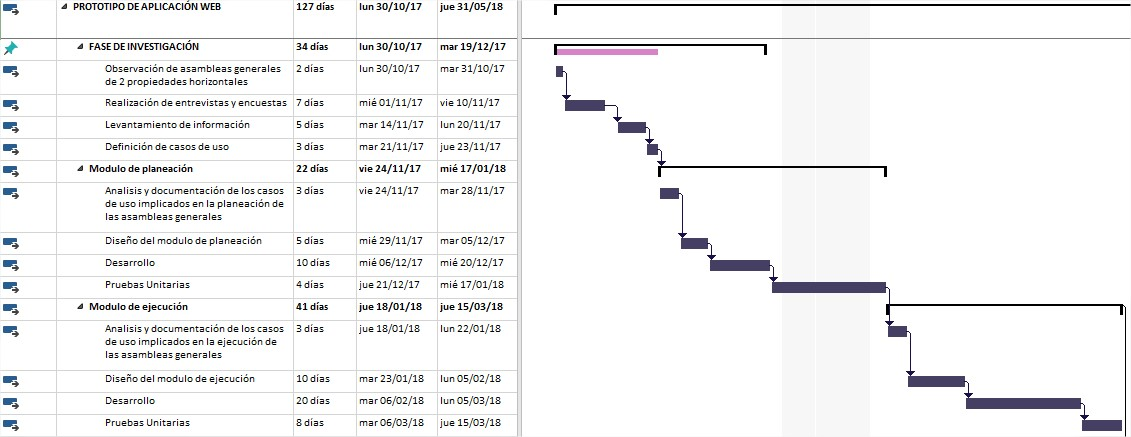
\includegraphics[width=16cm,height=8cm]{contexto/proyecto/imgs/Cronograma_parte1.jpg}
	\caption{Cronograma parte 1}{\scriptsize \textbf{Fuente:} Imagen propia}
\end{figure}
\vspace{1cm}
\begin{figure}[th!]
	\centering
	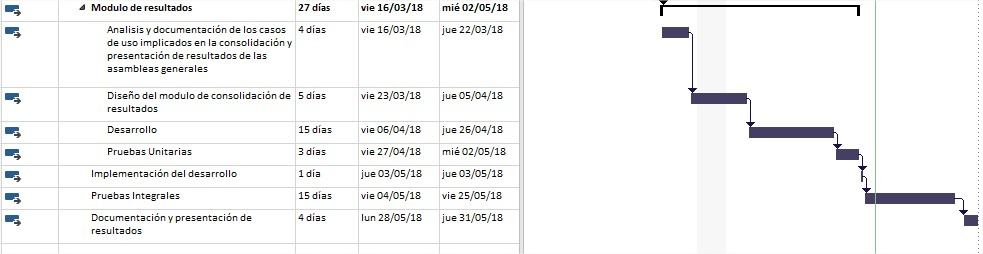
\includegraphics[width=13cm,height=4cm]{contexto/proyecto/imgs/Cronograma_parte2.jpg}
	\caption{Cronograma parte 2}{\scriptsize \textbf{Fuente:} Imagen propia}
\end{figure}

\section{Estudios de sistemas previos}

Realizando la verificación de la exitencia de otros sistemas que ofrecieran los servicios que se pretenden realizar en el desarrollo del proyecto se encontró una herramienta que permite la ejecución de las asambleas generales pero no entra en el proceso administrativo de las propiedades horizontales, este sistema se basa en el alquiler de dispositivos de votación basados en un control remoto que permite realizar la votación de manera electrónica, así mismo genera el control de asistencia, grabación del evento y alquiler de sonido. Lo anterior presenta una gran ayuda a la ejecución de asambleas generales de propiedad horizontal pero de igual forma es un gasto adicional a los ya incurridos dentro de los gastos administrativos.

Actualmente no se cuenta con sistemas propios que generan la ayuda mencionada anteriormente y sean propiedad de cada conjunto residencial.

\vspace{1.5cm}

\begin{figure}[th!]
	\centering
	
\includegraphics[width=9cm,height=5cm]{contexto/proyecto/imgs/puerta_enlace.jpg}
	\caption{Sistema Puerta de Enlace}{\scriptsize \textbf{Fuente:} Puerta de enlace  https://www.puertadeenlace.com/servicios/para-asambleas-todo-lo-necesario}
\end{figure}

\newpage